\documentclass[12pt]{jsarticle}
\pagenumbering{arabic}
\usepackage{listings,jlisting}
\usepackage{url}
\usepackage[dvipdfmx]{graphicx}
\usepackage{amsmath}
\usepackage{cases}

\lstset{
  language=,
  basicstyle={\small},%
  identifierstyle={\small},%
  commentstyle={\small\itshape\color[rgb]{0,0.5,0}},%
  keywordstyle={\small\bfseries\color[rgb]{0,0,1}},%
  ndkeywordstyle={\small},%
  stringstyle={\small\ttfamily\color[rgb]{1,0,1}},
  frame={tb},
  breaklines=true,
  columns=[l]{fullflexible},%
  numbers=left,%
  xrightmargin=0zw,%
  xleftmargin=3zw,%
  numberstyle={\scriptsize},%
  stepnumber=1,
  numbersep=1zw,%
  lineskip=-0.5ex%
}

\begin{document}

今回の課題では図\ref{fig:kairo}の回路に流れる電流の値をガウスの消去法、ヤコビ法、ガウスザイデル法を用いて求めることを目的とする。
\begin{figure}[h]
	\centering
	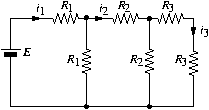
\includegraphics[clip,width=5.0cm]{./kairo.png}
	\caption{電流の値が不明な回路図}
	\label{fig:kairo}
\end{figure}

$E = 20[V], R_1 = 20[\Omega], R_2= 10[\Omega], R_3 = 17[\Omega] となっている。これらをもとにしてi_1, i_2, i_3 を求める。$

これらから連立方程式を立てると
\begin{eqnarray}
	\begin{cases}
		2R_1i_1 - R_1i_2 = E & \\
		R_1i_1 + 2R_2i_2 - R_2i_3 = E & \\
		R_1i_1 + R_2i_2 + R_3i_3 = E
	\end{cases}
\end{eqnarray}

$i$について整理すると
\begin{eqnarray}
	\begin{cases}
		i_1 = \frac{E + R_1i_2}{2R_1} &\\
		i_2 = \frac{E -R_1i_1 + R_2i_3}{2R_2} &\\
		i_3 = \frac{E -R_1i_1 - R_2i_2}{2R_2}
	\end{cases}
\end{eqnarray}

これらの式を用いて$i$について求める。

\section{課題1}
\subsection{ヤコビ法を基にしたガウスザイデル法の作製}
まずヤコビ法を実装したプログラムを(\cite{yacobiurl}から引用)をソースコード\ref{lst:yacobi}に示す。

\begin{lstlisting}[caption=yacobi.c,label={lst:yacobi}]
/*
  Yacobi  method
*/

#include <stdio.h>
#include <math.h>
#define n 4
#define n1 5
#define EPS 1.0e-15
#define KMAX 100

main()
{
	int i,j,k=0,l;
	double a[n1][n1],b[n1],x[n1],xn[n1],eps_sum;
	
		a[1][1]=4;  a[1][2]=1;  a[1][3]=0;  a[1][4]=-2;
		a[2][1]=1;  a[2][2]=4;  a[2][3]=-1; a[2][4]=1;
		a[3][1]=0;  a[3][2]=-1; a[3][3]=4;  a[3][4]=-1;
		a[4][1]=-2; a[4][2]=1;  a[4][3]=-1; a[4][4]=4;
		b[1]=5,     b[2]=-5,    b[3]=6,     b[4]=8;
		x[1]=0,     x[2]=0,     x[3]=0,     x[4]=0;
	
	do{
		eps_sum=0.0;
		for(i=1; i<=n; i++){
			xn[i]=b[i];
			for(j=1; j<=n; j++){
				if(j!=i) xn[i] -= a[i][j]*x[j];
			}
			xn[i] /=a[i][i];
		}
		for(i=1; i<=n; i++){
			eps_sum +=fabs(xn[i]-x[i]);
			x[i]=xn[i];
		}
		k++;
	}while(eps_sum>EPS && k< KMAX);
	if(k == KMAX){
		printf("Error!! The answers is not found.\n");
	}else{
		printf(" Iteration K = %d \n",k);
		for(i=1; i<=n; i++){
			printf( "x[%d] = %f ",i,x[i]);
		}
		printf(" \n");
	}
}
\end{lstlisting}
\subsection{ガウスザイデル法の作製}
ソースコード\ref{lst:yacobi}を基にして、ガウスザイデル法のプログラムを作製する。ヤコビ法とガウスザイデル法との大きな違いとして、ガウスザイデル法では今現在わかっている最新の変数の値を基に変数を求めることが挙げられる。ソースコード\ref{lst:gauss-seidel}にガウスザイデル法を示す。
\begin{lstlisting}[caption=gauss-seidel.c,label={lst:gauss-seidel}]
/*
  Gauss-seidel method
*/

#include <stdio.h>
#include <math.h>
#define n 4
#define n1 5
#define EPS 1.0e-15
#define KMAX 100

main()
{
	int i,j,k=0,l;
	double a[n1][n1],b[n1],x[n1],xn[n1],eps_sum;
	
		a[1][1]=4;  a[1][2]=1;  a[1][3]=0;  a[1][4]=-2;
		a[2][1]=1;  a[2][2]=4;  a[2][3]=-1; a[2][4]=1;
		a[3][1]=0;  a[3][2]=-1; a[3][3]=4;  a[3][4]=-1;
		a[4][1]=-2; a[4][2]=1;  a[4][3]=-1; a[4][4]=4;
		b[1]=5,     b[2]=-5,    b[3]=6,     b[4]=8;
		x[1]=0,     x[2]=0,     x[3]=0,     x[4]=0;
	
	do{
		eps_sum=0.0;
		for(i=1; i<=n; i++){
			xn[i]=b[i];
			for(j=1; j<=n; j++){
				if(j!=i) xn[i] -= a[i][j]*x[j];
			}
			xn[i] /=a[i][i];
			eps_sum +=fabs(xn[i]-x[i]);
			x[i]=xn[i];
		}
		k++;
	}while(eps_sum>EPS && k< KMAX);
	if(k == KMAX){
		printf("Error!! The answers is not found.\n");
	}else{
		printf(" Iteration K = %d \n",k);
		for(i=1; i<=n; i++){
			printf( "x[%d] = %f ",i,x[i]);
		}
		printf(" \n");
	}
}
\end{lstlisting}
改変点としてソースコード\ref{lst:yacobi} の34〜35行を31行のあとに移動した。ソースコードの量が少なくなった。
\section{課題2}
では実際にプログラムを使用し、iについて求めていく。
\subsection{課題2の結果}
\subsection{考察}
\subsection{使用したプログラム}
ソースコード\ref{lst:answer}にガウスの消去法、ヤコビ法、ガウスザイデル法を用いて求めた結果を出力するプログラムを示す。なお、このプログラムは上記のソースコード\ref{lst:yacobi}、\ref{lst:gauss-seidel}及び\cite{gaussian}のプログラムを引用、改変したものである。

\begin{lstlisting}[caption=answer.c,label={lst:answer}]
\end{lstlisting}



\begin{thebibliography}{9}
	\bibitem{yacobiurl} 片山英昭 ヤコビ法ソースコード \url{http://moodle.maizuru-ct.ac.jp/moodle/file.php/184/yacobi.c}
	\bibitem{gaussian} 片山英昭 ガウスの消去法ソースコード \url{http://moodle.maizuru-ct.ac.jp/moodle/file.php/184/gauss_pivot.c}
\end{thebibliography}
\end{document}

